
\begin{figure}[t]
    \centering
    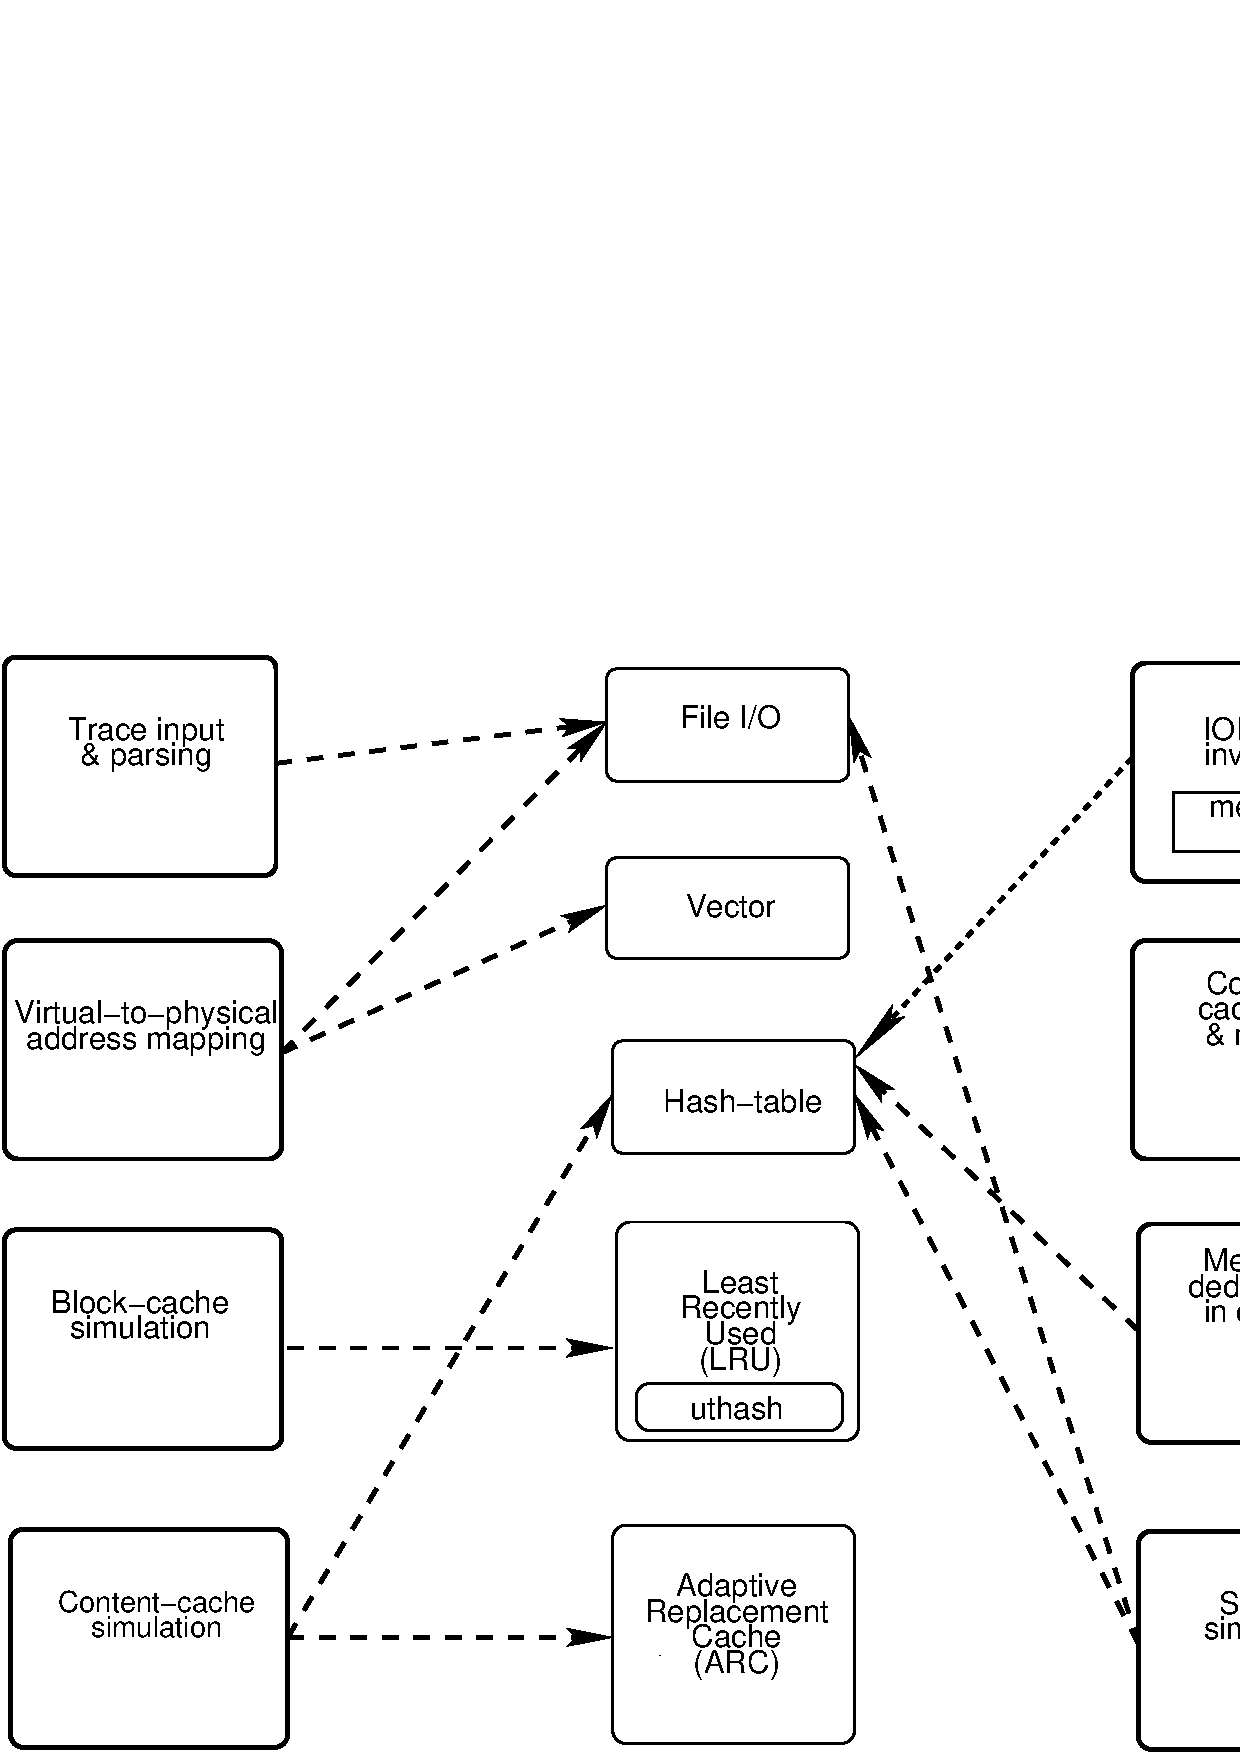
\includegraphics[scale=0.6]{simreplaychap-figures/simreplay-lowlevel.pdf}
%    \vspace{-0.1in}
    \caption{Low-level design of simulator: \textit{The left-most and the 
		right-most columns are the high-level components presented in 
		Fig.~\ref{fig:simreplay-interaction} and the center column contains
		the lower-level design components which underlie the
		higher-level design (as indicated by the unidirectional arrows).}}
    \label{fig:simreplay-lowlevel}
%    \vspace{-0.2in}
\end{figure}

Fig.~\ref{fig:simreplay-lowlevel} depicts the lower-level design for
each module specified in the earlier design diagram of 
Fig.~\ref{fig:simreplay-interaction}. In this section, we describe the
details of implementation of each of these modules in our simulator.

\subsection{Trace input \& parsing} 
\label{sec:simreplay-parsing}
%\subsection{Per-VM block requests}
%\paragraph{Input trace file format.} 
The trace files present at \cite{iodedup-online} has the following
format for every request:-
\begin{verbatim}
    [ts in ns] [pid] [process] [lba] [size in 512 Bytes blocks] [Write or 
	Read] [major device number] [minor device number] [MD5 per 4096 Bytes]
\end{verbatim}
The last column of the above format is in terms of the hexadecimal 
representation of the MD5 of the content. Hence, all above fields have
content in deterministic range, and parsing of the trace file can
be performed in a straight-forward line-by-line fashion. 

The above trace files represent a single workload each\textemdash{}\textit{webvm},
\textit{homes} or \textit{mail}, as mentioned earlier. However, our 
simulator is meant to simulate the replay of block requests of multiple
VMs on a single host. Hence, we accommodate an additional attribute, a VM
identifier, within each record in the trace. Accordingly, the 
data-structure representing a single request within the simulator is
as shown in Listing \ref{lst:vmreq}.

%\subsection{Parsing the input trace file}

\lstset{language=C,
	caption={Data-structure representing a single request.},
	label=lst:vmreq
}
\begin{snippet}
/* @vmname:  VM identifier
 * @time:    Time stamp when trace was emitted
 * @block:   VM I/O block identifier
 * @bytes:   Number of bytes transferred
 * @content: Content to be transferred
 * @rw:      Read (1) or write (0) 
 */
struct vmreq_spec {
    char vmname[HOSTNAME_LEN];
    __u64 time;
    __u32 block;
    __u32 bytes;
    __u8 *content;
    unsigned char rw:1;
};
\end{snippet}

\subsection{Addressing trace file inconsistencies by storage simulation}
\label{sec:simreplay-simdisk}
The trace files present at \cite{iodedup-online} have
the content (or rather, MD5 hash representation of content) along-with every read
and write request. This implies that a replay performed at a later
date can rely on these content for simulating storage reads and writes,
without having to actually perform the I/O on storage. However, our
experience with usage of these traces revealed that there were 
inconsistencies in the content reported in the traces. 

We define trace \textit{inconsistency} as the case where a piece of 
content was reportedly
read from or written to a block, but the next read request to the same
block reports another piece of content, although there were no writes to
that block in the interim. This could be caused due to some missing 
records in the trace. However, to evaluate the correctness of any 
replay module, the traces themselves would have to be consistent. Hence,
in our simulator, we maintain a simulated storage wherein the block
content is written to a file, and can be read back when required. In
this model, the first access to every block (whether read or write) is 
considered as the ground truth and written to the file (i.e. simulated 
storage). 
Naturally, subsequent write requests do not face any issues of consistency, 
since they are just new data to be written to storage.
However, for every subsequent read request, the content present on 
simulated storage is used for replay (since it is the consistent version), 
instead of
the content present in the trace (since it was found to be inconsistent 
at times).

\begin{figure}[t]
    \centering
    \includegraphics[scale=0.6]{simreplaychap-figures/simreplay-simdisk.pdf}
%    \vspace{-0.1in}
    \caption{Implementation of storage simulation in custom simulator. Each 
			hash-table entry contains an offset into the 
			\textit{simdisk} file.}
    \label{fig:simreplay-simdisk}
%    \vspace{-0.2in}
\end{figure}

The implementation of storage simulation in the custom simulator involves
usage of hash-tables and file I/O, as indicated in 
Fig.~\ref{fig:simreplay-lowlevel}. The file I/O module is required
because a file (referred as \textit{simdisk}) 
is used to store the content (or MD5 hash of content). 
Additionally, to enable ``storage-lookup'' using the block address,
we use a hash-table with the block address (string formatted) as the key.
Fig.~\ref{fig:simreplay-simdisk} presents a pictorial view of 
how storage simulation is implemented in our simulator.
Within the hash-table entry that is identified for a given block, we 
maintain a file offset value which indicates the offset within the 
\textit{simdisk} file, at which the corresponding content is stored.

\subsection{Mapping from virtual disk space to physical disk space}
As mentioned in Section~\ref{sec:simreplaychap-v2p},
the input V2P mapping
indicates the range of physical blocks (i.e. blocks on host storage)
that map to the address space of each VM (i.e. blocks of virtual disk)
for simulation. 
For a trace replay file that has a single VM's requests, 
this input file is not mandatory, since the simulator can infer this map
dynamically from the trace file itself. 
In fact, at the end of the 
simulator invocation, the inferred V2P map is output to the same
file. Thus, with a single-VM trace file, it is possible to determine
the range of blocks (i.e. maximum block number accessed) for that VM.
However, in case of a trace input
file that has aggregated requests from multiple VMs, this input file is 
mandatory and it is validated that the ranges of blocks specified for 
each VM does not overlap with the range of any other VM. 
In order to
build this multi-VM input V2P file, the output V2P file(s) from the single-VM
trace executions can be used additively, as indicated in 
Section \ref{sec:simreplaychap-v2p}.

The input of V2P mapping requires the file 
I/O module (refer Fig. \ref{fig:simreplay-lowlevel}) since the mapping
has to be read from and written to a file. Also, after receiving the 
input mapping, the simulator uses a vector data-structure for storing
the 3-tuples for each VM involved in replay.
The \textit{vector} data-structure is basically the same as an array, 
except that it can grow as required, unlike an array which has static
size allocation.

%\subsection{Enabling input of mapping}
%A file can be specified using option -m which should contain a 3-tuple of
%above format per line. Each line is for one VM. 
%\subsection{Implementation}
%Using vectors to store a 3-tuple consisting of \textit{vmname},
%base block address per VM, and capacity per VM.

\subsection{Block-cache simulation}
%\subsection{Implementation details}
Since the block-cache needs to be looked-up by block ID, a hash-table
implementation is required. Also, since the LRU policy has to be applied
to the elements in the block-cache, all such elements should also form
part of a linked list. Instead of implementing this cache from scratch,
we used an existing hash-table implementation called 
\texttt{uthash}\cite{uthash}, which is basically a hash-table for 
storing C data-structures. It requires that a \textit{UT\_hash\_handle}
element be added to the data-structure that is to be stored into the
hash-table and another field (say blockID) of the same data-structure 
can be used as the key to lookup the hash-table. 

The \texttt{uthash}
module also maintains a linked list of all the elements in the hash-table
in ``insertion'' order. In order to simulate LRU policy for the
block-cache, we have to tweak the ordering slightly, as follows.
If a block is already present in the hash-table, inserting it again
for the same key is an error in the \texttt{uthash} module. Modifying it 
in-place is not an error though, but it will not cause the LRU ordering
that we require. So, when we find that the block being requested is in cache,
we first delete it from the hash-table, and then re-insert it,
to simulate LRU ordering.

\subsection{IODEDUP metadata store}
In our simulator, we have designed and implemented the IODEDUP metadata
store in a similar fashion as the DRIVE metadata store except for two 
major differences: (i)~The DRIVE metadata store is present within the
virtual address space whereas the IODEDUP metadata store holds mapping
within the physical storage address space, (ii)~The DRIVE metadata store
maintains implicit caching hints to aid in request redirection whereas IODEDUP
metadata store is used to retrieve the content hash which is further used
for content-cache lookup.

\subsection{Content-cache simulation}
The content-cache is implemented using a hash-table implementation,
and has the Adaptive Replacement Cache (ARC) as the cache replacement
policy. The ARC policy basically maintains four lists\textemdash{}(i) a list of
in-cache elements in the LRU order, (ii)~a list of in-cache elements
in the LFU order, (iii)~a list of recently-evicted (ghost) elements 
in the LRU order, and (iv)~a list of ghost elements in the LFU order.
The ARC algorithm uses these four lists and maintains their relative
sizes in order to most effectively keep the most recently used and
the most frequently used elements in cache. 

In our implementation, we use an online implementation of the ARC
algorithm for the content-cache simulation. The content-cache can
be looked up based on the hash of the content, and the insertion/deletion
in cache is performed according to ARC policy mentioned above.
For a read request, the content-cache needs to be looked up only
upon a metadata hit in the IODEDUP system. In case of a metadata
miss, the read request is forwarded to the storage instead.
For a write request, the content-cache is written into and the
metadata is updated accordingly. The content-cache is maintained
with write-through semantics, as specified in~\cite{iodedup}.

\subsection{Quantifying content-deduplication in cache(s)}
The aim of this simulator is to study cache management effectiveness,
and we quantify the content deduplication effected within the cache(s) 
(including the content-cache as well, for IODEDUP)
as a measure of its effectiveness. In our simulator, we simulate 
traps at every block insertion and eviction from cache(s).
A separate hash-table is maintained which keeps track of the duplicate
content among the blocks currently present in the simulated cache(s), 
and this hash-table is modified at every such interrupt/trap occurrence.

In case of a block being inserted into the cache, in the trap
that ensues, we fingerprint it 
and lookup the hash-table to see if there are any other blocks already
in cache(s) with the same fingerprint. If so, its reference counter is
incremented. When a block is evicted from cache, the trap processing
again involves fingerprinting it and searching the hash-table. If
the content is present in the hash-table, its reference counter is 
decremented, and the entry is removed from the hash-table if the 
reference counter reaches value of zero.
At any instance during replay, the \textit{content deduplication factor}
can be defined as the ratio of number of unique blocks in cache(s) to 
number of total blocks in cache(s). Higher the content deduplication
factor, higher the efficiency of the cache space utilization, and hence
higher the storage access performance.


\subsection{Verifying the correctness of the simulator}
To ensure correctness of the simulator, each individual module was
first unit-tested manually with small input sizes, and then the entire
module as a whole was integration-tested with whole trace files. 
For every block that is present in cache (whether block-cache 
or content-cache), it is verified that the content present on the 
simulated storage is actually the same as the content returned from
cache. Note that this is only a simulation-correctness check and does not 
count towards number of disk reads for replay.
Additionally, for each invocation of the simulator, the following are 
verified in code (using assert statements).
\begin{itemize}
\item The total number of \textit{reads} replayed equals the sum of 
\textit{cache hits} and \textit{cache misses}.
\item The total number of \textit{cache hits} equals the sum of 
\textit{read cache hits} and \textit{write cache hits}.
\item The number of \textit{read cache misses} equals the number
of \textit{disk reads}.
\item The number of \textit{read cache misses} equals the sum of
\textit{compulsory} and \textit{capacity misses}.
\item The total number of \textit{writes} replayed equals the total number
of blocks written to disk.
\end{itemize}
